%\begin{figure}[ht]
%\vskip 0.2in
%\begin{center}
%\centerline{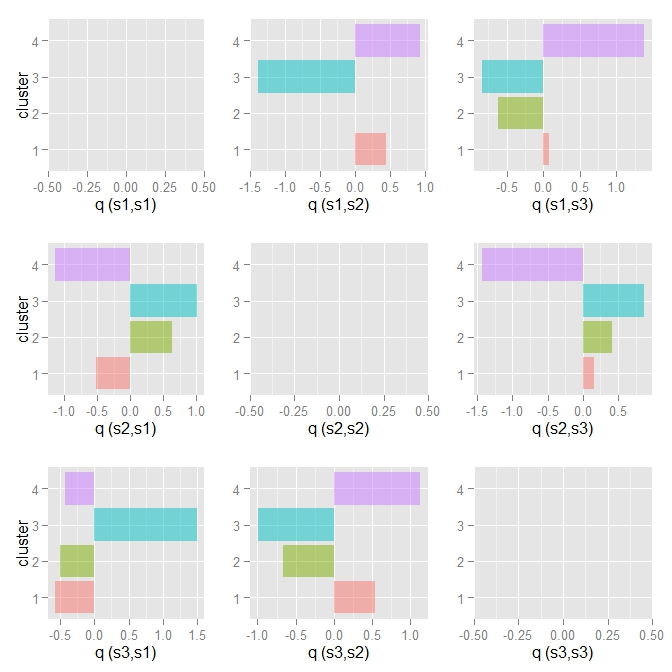
\includegraphics[width=\columnwidth]{fig/qmatrix.jpeg}}
%\caption{Historical locations and number of accepted papers for International
%  accepted papers for ICML 2008 was unknown and instead estimated.}
%\label{icml-historical}
%\end{center}
%\vskip -0.2in
%\end{figure}
 Using biopsy results as a gold standard for clustering, our results indicate over a 20\% relative improvement on a benchmark (.41-.51 b-cubed) for detecting liver fibrosis in a subset of hepatitis C patients from the liver disease data.  Relative to the results based on the whole data set, better performance is achieved for the hepatitis C patients without interferon therapy.  This is not surprising.  Interferon therapy is physiologically disruptive and the reason for the selection criteria in the benchmark set.  However, despite the introduction of this noise, our method performs better on the group of all patients than the benchmark performs on only this subset of more predictable patients.

Of clinical relevance was an `extreme' effect that could be viewed among different clustering runs.  The lowest risk cluster, designated by the highest proportion of patients with no or minor fibrosis, reported 80-94\% purity and was composed of 15-25 percent of the patients for a $4<k<6$.  This cluster represents patients with very low risk of fibrosis, and may be good candidates for delaying biopsy.

Additionally, for an inpatient population, we can detect recognizable differences in the incidence of physicians' orders for glucose tests among discovered groups that can be visualized. We also assess the performance of pairing temporal abstraction with a non-parametric Bayesian clustering.  It conveniently eliminates the need to estimate $k$, and  performed better that spectral clustering on the hepatitis data set.

The glucose test experiment demonstrates two distinct groups with average silhouette value of .73 and .88 and accounting for almost 60\% of the population sampled.  These two groups show the most dramatic differences in average sequence entropy (0.05-0.14), the fraction of days measured (0.01-0.04) and the number of tests (8.60-39.64).  When the original sequence is viewed as a heat map, a typical patient's sequence in the low risk group will consists of sparse signals, with only the initial visit consisting of more that one contiguous tests.  However, patients in group have testing patterns that are longer in duration, showing streaks of contiguous testing, and suggesting they are more prone to diabetes related morbidity.  Patients in the remaining clusters represent an intermediate between these two groups and mixtures of testing patterns.

Since diabetes is undiagnosed in millions of Americans, and preventative treatment can help avoid serious effects and avoidable costs to providers, using administrative data, such as glucose testing pattern, may prove useful for disease surveillance.  For example, an insurance provider does not have access to lab results, but they will have a signal for per patient tests, information on demographic risk factors, and other billing diagnoses for patients. The ability to leverage high level signals with demographic and other claims data to flag prediabetes or undiagnosed diabetes could be useful for developing cost-savings strategies that improve health outcomes in parallel.
